% ============ Appendices ============
\section{LLM Scoring Prompt}\label{app:prompt}

The following system prompt was applied verbatim to every batch of 25 headlines in all conditions; the named and repeat conditions prefix each headline with ``[Company]'', and the anonymized condition presents the de-identified headline text with no prefix. The scoring model is \texttt{glm-4-plus} (Z.ai), accessed through its API. Every request disables the model's extended-reasoning (``thinking'') mode~---a request-level switch that turns off chain-of-thought generation before the answer, forcing direct output~---and otherwise uses the provider's default decoding parameters: no temperature, top-$p$, or seed overrides, so the sampling distribution is whatever the endpoint defaults to, and its stochasticity is a measured property of the instrument (Section~\ref{sec:results:h3}) rather than an assumption. Batches that failed to parse were retried up to three times. All raw responses and batch logs are archived in the replication package.

\begin{quote}
\footnotesize\ttfamily\raggedright\setlength{\parindent}{0pt}
You are an expert financial analyst specialized in news
sentiment analysis for equity research. You evaluate how news
headlines affect a company's stock value.\par
\vspace{4pt}
For each headline you must return:\par
- "sentiment": integer from -100 to +100. -100 = extremely
  negative impact on the company's stock value; 0 = neutral or
  no clear impact; +100 = extremely positive impact.
  Judge from the perspective of a shareholder of the company.\par
- "relevance": integer from 0 to 100. 100 = headline is
  directly about the company's business, earnings, products,
  guidance, or stock; 0 = headline mentions the company only
  incidentally or is a generic market/quote page.\par
\vspace{4pt}
Rules:\par
- Base your judgment ONLY on the information in the headline text.\par
- Earnings beats, raised guidance, product launches,
  upgrades, buybacks = positive.\par
- Earnings misses, cut guidance, lawsuits, recalls,
  downgrades, layoffs = negative.\par
- Speculation or rumor framing lowers the magnitude toward zero.\par
- Generic quote pages, price summaries without direction, or
  calendar pages = sentiment 0, relevance low.\par
\vspace{4pt}
Return ONLY a valid JSON array. One object per headline, in
the same order as given, with fields: "id", "sentiment",
"relevance". No other text.
\end{quote}

\section{Anonymization Procedure}\label{app:anon}

Company identifiers are removed by a case-insensitive alias table mapping each firm's name, common short forms, and ticker to the phrase ``the company'' (e.g., ``Apple Is Up 20\% in 2026. What Will It Take for AAPL Stock'' becomes ``the company Is Up 20\% in 2026. What Will It Take for the company Stock''). 325 of 341 in-window headlines (95.3\%) are altered. The procedure is conservative: product names, third-party firms mentioned inside a headline, and stylistic cues are left intact, so the anonymized condition is a lower bound on de-identification. Quantifying the residual firm-identity component under the executed alias table: 5 of 341 anonymized headlines (1.5\%) still name at least one other sample firm~---under both a case-insensitive and a case-sensitive matching convention~---with analyst actions (``BofA,'' ``Morgan Stanley'') and co-mentioned mega-caps the typical cases. The dominant de-identification gap is therefore product language (e.g., device or franchise names) rather than residual firm names. Ambiguous tickers that collide with common words (e.g., ``COST,'' ``CAT,'' ``V'') are replaced only in their exact all-caps form.

\paragraph{A disclosed failure of the procedure.} The executed alias table contains no entry for ticker V (whose identifiers would have been ``Visa''), and all ten in-window V headlines contain the word ``Visa'' but never the standalone all-caps token ``V.'' The anonymization was therefore a no-op for those ten headlines: the text sent to the model under the anonymized condition still named the focal company~---2.9\% of the 341~---and the condition contrast for them is effectively named-versus-named. Five of the ten are U.S.\ State Department ``Visa Bulletin'' immigration headlines (unrelated to the payments company; all scored at relevance 20, so they never enter the firm-day sample but do enter the article-level tests), and five enter the relevance-qualified sample. The failure is instructive in two ways. First, it materially moves the marginal same-session identity contrast: excluding the ten V headlines sharpens it from $-1.04$ ($p=0.11$) to $-1.29$ ($p=0.04$; Wilcoxon $p=0.03$), which is why Section~\ref{sec:results:h2} reports the contrast as a range rather than a verdict. Second, and more generally, it was caught only by re-running the anonymizer with a verification pass~---checking that anonymized text no longer matches the focal firm's identifiers~---which we now treat as a mandatory step of the protocol rather than an optional one. The illustrative pair: the named condition ``[Visa] Visa Stock Just Posted Its Best Quarter Since 2022.'' scored $+80$ (relevance 90), while the ``anonymized'' condition~---the identical text minus the prefix~---scored $0$; the difference is a clean single-headline demonstration of how much identity information the prefix-plus-name carries. Computed by \texttt{v\_exclusion.py} from the archived corpus and scores.

\section{Firm-Level Coverage}\label{app:coverage}

Table~\ref{tab:coverage} reports news coverage by firm: in-window headlines and relevance-qualified trading-day firm-days. Coverage ranges from 4 to 17 articles per firm and correlates with firm prominence in web search, which motivates the selection analysis of Section~\ref{sec:results:h5} and the size interaction of Appendix~\ref{sec:appaux}. The table is generated directly by \texttt{coverage\_table.py} from the archived corpus, scoring, and panel files, so every cell is reproducible; the generator asserts that the rendered cells show each of the 36 firms exactly once and that the column totals equal the verified corpus totals (341 in-window articles, 240 relevance-qualified trading-day firm-days).

% AUTO-GENERATED by scripts/coverage_table.py -- DO NOT EDIT BY HAND
% Verified: 36 tickers, column sums 341 / 240
\begin{table}[tbp]
\centering
\small
\caption{News coverage by firm (in-window articles and trading-day firm-days)}
\label{tab:coverage}
\begin{adjustbox}{max width=\textwidth}
\begin{tabular}{lrr@{\hskip 1.6em}lrr@{\hskip 1.6em}lrr}
\toprule
Ticker & Articles & Firm-days & Ticker & Articles & Firm-days & Ticker & Articles & Firm-days \\
\midrule
AAPL & 16 & 9 & GE & 8 & 6 & MSFT & 10 & 5 \\
ADBE & 10 & 9 & GOOGL & 6 & 4 & NFLX & 14 & 11 \\
AMD & 13 & 8 & GS & 11 & 7 & NVDA & 13 & 8 \\
AMZN & 8 & 6 & IBM & 8 & 7 & ORCL & 12 & 9 \\
AVGO & 13 & 10 & INTC & 14 & 11 & PFE & 5 & 4 \\
BA & 5 & 4 & JNJ & 7 & 4 & PG & 6 & 4 \\
BAC & 7 & 5 & JPM & 4 & 4 & QCOM & 7 & 7 \\
CAT & 6 & 5 & KO & 10 & 6 & TSLA & 9 & 8 \\
COST & 15 & 11 & LLY & 6 & 6 & V & 10 & 3 \\
CRM & 17 & 8 & MA & 9 & 8 & WFC & 12 & 9 \\
CVX & 7 & 5 & META & 11 & 7 & WMT & 13 & 9 \\
DIS & 4 & 4 & MS & 7 & 2 & XOM & 8 & 7 \\
\bottomrule
\end{tabular}
\end{adjustbox}
\begin{tablenotes}[flushleft]\footnotesize
\item Articles: headlines dated 2026-07-01 to 2026-10-14 in the archived corpus (column total 341). Firm-days: unique firm--date cells with scored relevance $\geq$ 30 falling on a trading date (column total 240, equal to the regression sample). 36 firm--date cells fall on non-trading dates and are dropped without roll-forward (Section~\ref{sec:data}). Computed by \texttt{coverage\_table.py} from \texttt{news\_all.json}, \texttt{llm\_scores.json}, and \texttt{panel.csv}.
\end{tablenotes}
\end{table}


\section{Auxiliary Analyses}\label{sec:appaux}

This appendix reports the three descriptive exercises summarized in Section~\ref{sec:robust:aux}: the horizon path, the portfolio sorts, and the heterogeneity interactions. None is part of the declared test family; each is reported under the audit's inference standard.

\subsection{The horizon path, re-read}

The horizon path shows a sign pattern~---positive at $t+1$ ($t=2.10$), negative at $t+2$ ($t=-2.04$, $p=0.042$), fading by $t+3$ ($t=-1.52$)~---that invites an attention-driven overshooting-and-correction reading. The audit re-reads the pattern rather than discarding it. A subsample selected on high absolute returns (H5) and scored with text that partially echoes those returns (H4) mechanically produces short-horizon continuation followed by reversal: this is the classical news-event return dynamics documented by \citet{chan2003} for reasons (liquidity provision, bid--ask bounce, order-flow imbalance) that require no sentiment semantics at all. Under the decomposition~\eqref{eq:score}, the observed path is what $\rho>0$ plus event-selection generates; the reversal is therefore \emph{consistent with} the echo channel and does not independently identify overshooting. We accordingly read the reversal as a pattern consistent with the echo interpretation rather than as an independent finding, and note that the next-day open-to-close coefficient is small and insignificant ($t=0.45$)~---better read as the echo's asymmetry between the overnight and intraday windows on an underpowered sample than as evidence of overnight diffusion.

\subsection{Portfolio sorts, honestly reported}

Sentiment-sorted quintile portfolios on the baseline sample earn $-20.3$, $+18.9$, $+6.5$, $+35.0$, and $+69.6$ \bps{} from Q1 to Q5, a Q5$-$Q1 spread of 89.9 \bps{} with a Welch $t=1.24$ ($p=0.22$). Three facts deserve equal prominence: the sort is \emph{not monotone} (Q2 exceeds Q3); the spread is not statistically significant; and the IC and direction tests are null (mean daily IC $+0.035$, $t=0.30$ over 25 usable cross-sections; direction logit $p=0.20$, marginal effect 11.5 points). Under the audit's standard, the economic-significance evidence does not clear its own bar, and gross-of-cost spreads on an event-selected sample of 47 observations per quintile should not be quoted as tradable. No transaction-cost claim is made beyond the observation that any cost level above zero further erodes a statistically insignificant spread.

\subsection{Heterogeneity: interactions, not splits}

A split-sample presentation~---coefficient significance in above- versus below-median subsamples~---is the natural first pass at heterogeneity, and it is the rhetoric the econometrics literature warns against, since separate significances do not test a difference. Table~\ref{tab:inter} reports the formal interaction-term tests. The size interaction is significant ($t=2.25$, $p=0.025$): predictability genuinely concentrates in above-median-dollar-volume firms, which in this corpus is nearly mechanical~---mega-caps dominate search coverage, so the instrument is most precise (densest text input) exactly there. The news-intensity interaction is marginal ($t=1.90$, $p=0.057$). The volatility interaction is zero ($t=0.01$): a volatility-regime split showing coefficients that differ by 0.0007 across regimes with different standard errors implies no detectable interaction, so no state-dependence claim survives a formal test. Figure~\ref{fig:hetv2} contrasts the two inference styles directly~---the point of the exercise is methodological as much as substantive.

\begin{table}[htbp]
\centering
\small
\caption{Heterogeneity: formal interaction tests versus split-sample statistics}
\label{tab:inter}
\begin{threeparttable}
\begin{tabular}{lccc}
\toprule
Channel & Interaction coefficient & $t$ & $p$ \\
\midrule
Sentiment $\times$ large firm (above-median dollar volume) & 0.0248 & 2.25 & 0.025 \\
Sentiment $\times$ multi-headline firm-day & 0.0512 & 1.90 & 0.057 \\
Sentiment $\times$ high-volatility regime & 0.0001 & 0.01 & 0.994 \\
\bottomrule
\end{tabular}
\begin{tablenotes}[flushleft]\footnotesize
\item Interactions from $r_{i,t+1} \sim \text{sentiment} + \text{sentiment}\times\text{modifier} + \text{modifier} + \text{same-day return} + \text{controls}$, two-way clustered, $N=205$. A volatility-regime split ($t=2.49$ vs.\ $t=1.00$) implies no detectable interaction.
\end{tablenotes}
\end{threeparttable}
\end{table}

\begin{figure}[htbp]
\centering
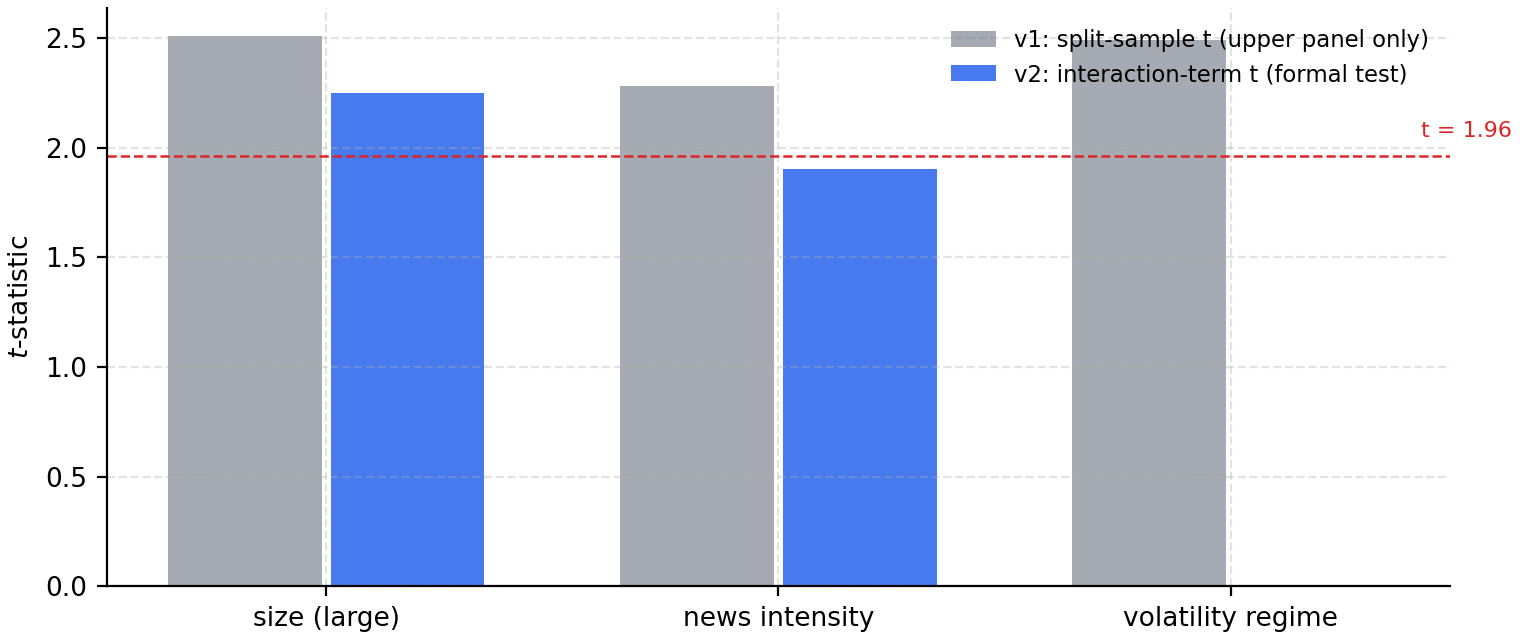
\includegraphics[width=0.8\textwidth]{../data/figures/fig_heterogeneity_v2.png}
\caption{Split-sample $t$-statistics (grey) versus formal interaction $t$-statistics (blue) for the three heterogeneity channels. Only the size effect survives formal testing; the volatility claim collapses to zero.}
\label{fig:hetv2}
\end{figure}

\section{Power and Minimal Detectable Effects}\label{app:power}

For each test in the declared family, Table~\ref{tab:power} reports the observed effect, its standard error, the two-sided 5\% minimum detectable effect at 80\% power ($\text{MDE}_{80} = (z_{0.975}+z_{0.80})\times\text{SE} = 2.80\times\text{SE}$), and the power of the test against the observed effect, $\Phi(|\delta|/\text{SE}-1.96)+\Phi(-|\delta|/\text{SE}-1.96)$. Standard errors for regression coefficients are the two-way clustered values of Table~\ref{tab:core}; standard errors for the difference tests are implied by the bootstrap confidence intervals of Table~\ref{tab:diff} (width divided by $2\times1.96$); the level-shift rows use their paired standard errors; the selection row uses the two-way clustered standard error of the fixed-effects specification of Section~\ref{sec:results:h5}, estimated on the $N=2{,}628$ firm-days with non-missing same-day returns (the 2,664-cell panel less the 36 first-trading-day cells, which lack a prior close and hence a same-day return). The table quantifies what the paper's non-rejections can and cannot rule out: the named-versus-anonymized predictive difference rules out substitutions larger than $0.006$~---about 42\% of the baseline coefficient itself~---while the named-versus-dictionary contrast rules out almost nothing ($\text{MDE}_{80}=0.094$, more than six times the baseline). At the return layer, the design can only detect next-day coefficients of $0.020$ or larger (72 \bps{} per one-standard-deviation sentiment move, against the observed 54 \bps{}), and the achieved power against the observed effect is 0.56: the marginal significance of H1 is exactly what an underpowered design produces around a true effect of this size. The H4 echo split has power 0.31 against its observed difference, which is why Section~\ref{sec:results:h4} labels it directional rather than established. At the measurement layer, the level-shift and selection tests are comfortably powered (0.999 and 0.79), which is the statistical counterpart of the paper's narrative: the channels the audit finds with confidence are the ones it can measure. The same-session identity row is the staged contrast: at $|\delta|=1.04$ points and $\text{SE}=0.65$, the design reaches power $0.36$~---the marginal mean-test result is what a design of this size produces around a one-point effect, and the rank test and V exclusion are the sharper instruments (Section~\ref{sec:results:h2}).

\begin{table}[htbp]
\centering
\small
\caption{Power and minimal detectable effects for the declared family}
\label{tab:power}
\begin{tabular}{lcccc}
\toprule
Test & Observed & SE & $\text{MDE}_{80}$ & Power \\
\midrule
H1: baseline next-day coefficient (named) & 0.0149 & 0.0071 & 0.020 & 0.56 \\
H2: $\beta_{\text{named}}-\beta_{\text{anonymized}}$ & 0.0004 & 0.0023 & 0.006 & 0.05 \\
H2: $\beta_{\text{named}}-\beta_{\text{dictionary}}$ & $-$0.0119 & 0.0335 & 0.094 & 0.07 \\
H4: $\beta_{\text{price-lang.}}-\beta_{\text{clean}}$ & 0.0436 & 0.0297 & 0.083 & 0.31 \\
H2: identity level shift (points, $n=341$) & 4.75 & 0.92 & 2.59 & 1.00 \\
H5: coverage selection (\bps, $n=2{,}628$) & 61.1 & 22.2 & 62.1 & 0.79 \\
H2: same-session identity shift (points, $n=341$) & $-$1.04 & 0.65 & 1.83 & 0.36 \\
H2: interleaved identity shift (points, $n=341$, session 3) & $-$2.82 & 1.03 & 2.88 & 0.78 \\
\bottomrule
\end{tabular}
\begin{tablenotes}[flushleft]\footnotesize
\item Two-sided 5\% tests; $\text{MDE}_{80}=2.80\times\text{SE}$. ``Power'' is achieved power at the observed effect. The identity-level-shift row is the cross-session contrast as declared; the same-session row is its staged re-estimate; the last row is the interleaved-session confirmatory contrast under the conservative batch-call-clustered SE (the headline-level SE of 0.66 would give power 0.99; the round-level meta-test is stronger still). The H4 and H5 rows use the $B=9{,}999$ bootstrap CI and the fixed-effects clustered SE of the panel inference specification. Computed by \texttt{revision\_power.py} (family and session-2 rows) and \texttt{analysis\_v3.py} / \texttt{reinference.py} (session-3 row) from archived artifacts.
\end{tablenotes}
\end{table}

\subsection{Equivalence Assessment of the Instrument Contrasts}\label{app:equiv}

Table~\ref{tab:power} runs the power logic one way~---what differences this sample could detect. The instrument conclusions require running it the other way as well: a non-rejected difference is not evidence of equivalence, and several statements a reader might naturally form (``the conditions are indistinguishable,'' ``the clean subsample shows no signal'') are equivalence claims wearing difference-test clothes. We therefore re-assess every predictive-coefficient contrast as a two-one-sided-tests (TOST) equivalence assessment on the same day-cluster bootstrap machinery as Table~\ref{tab:diff}, with $B=9{,}999$ resamples of the trading-day clusters (fresh seed) and the bootstrap's 90\% percentile interval as the test statistic: a contrast is equivalent at margin $\delta$ iff its entire 90\% interval lies inside $(-\delta, +\delta)$. The primary margin follows replication practice~---$\delta^{*}=0.0074$, one half of the benchmark named coefficient, the ``same order of magnitude'' standard: a predictive difference below half the effect itself cannot reverse any qualitative statement about the instrument, while a difference above it would mean the two conditions measure materially different signals. In response units, $\delta^{*}$ is 27 \bps{} of next-day return per one-standard-deviation firm-day sentiment shock (SD $0.361$), against a benchmark response of 54 \bps{}. Because a margin is a convention, each contrast's \emph{equivalence margin threshold} (EMT)~---the smallest margin at which it passes, i.e.\ $\max(|q_{5}|,|q_{95}|)$~---is reported alongside, so any reader-preferred margin can be tested by inspection. The margin rule was fixed before any verdict was computed; the analysis as a whole was designed in revision, after the difference tests were known, and is therefore labeled exploratory and reported outside the declared family (Section~\ref{sec:framework:inference}).

\begin{table}[htbp]
\centering
\small
\caption{Equivalence assessment (TOST) of predictive-coefficient contrasts}
\label{tab:tost}
\begin{adjustbox}{max width=\textwidth}
\begin{tabular}{lrrrrcl}
\toprule
Contrast & $\widehat{\Delta}$ & 90\% CI & EMT & EMT/$\hat\beta$ & Power & Verdict at $\delta^{*}$ \\
\midrule
Named $-$ anonymized (cross-session) & $+0.0004$ & $[-0.0035, +0.0040]$ & 0.0040 & 0.27 & 0.90 & Equivalent \\
Named $-$ anonymized (same-session) & $+0.0002$ & $[-0.0027, +0.0032]$ & 0.0032 & 0.21 & 0.99 & Equivalent \\
Named $-$ anonymized (interleaved) & $+0.0013$ & $[-0.0025, +0.0062]$ & 0.0062 & 0.42 & 0.74 & Equivalent \\
Named $-$ anonymized (session 5) & $-0.0018$ & $[-0.0052, +0.0021]$ & 0.0052 & 0.35 & 0.91 & Equivalent \\
Named $-$ swapped (session 5) & $-0.0039$ & $[-0.0083, +0.0004]$ & 0.0083 & 0.56 & 0.75 & Not established \\
Named $-$ LM dictionary & $-0.0119$ & $[-0.0658, +0.0415]$ & 0.0658 & 4.42 & 0.00 & Uninformative \\
Priced $-$ clean (echo split) & $+0.0436$ & $[+0.0005, +0.0976]$ & 0.0976 & 6.55 & 0.00 & Uninformative \\
Clean coefficient vs.\ zero & $+0.0033$ & $[-0.0071, +0.0136]$ & 0.0136 & 0.91 & 0.00 & Not established \\
\bottomrule
\end{tabular}
\end{adjustbox}
\begin{tablenotes}[flushleft]\footnotesize
\item $\widehat{\Delta}$: observed coefficient difference (next-day specification with controls; the echo rows use the same-day-control specification actually estimated). EMT: equivalence margin threshold, the smallest $\delta$ at which the percentile TOST passes, $\max(|q_{5}|,|q_{95}|)$ of the day-cluster bootstrap ($B=9{,}999$, seed 20261020). $\delta^{*}=0.0074$ (half the benchmark named coefficient; 27 \bps{} per one-SD shock). ``Power'': analytic power at a true difference of zero (bootstrap SE, $z_{0.95}=1.645$). Sample multiples needed for 80\% power at $\delta^{*}$: 0.5--1.1 for the four de-identification contrasts and the swap (the present sample meets or exceeds the requirement), 6.1 for clean-vs-zero, 143.7 for the echo split, 164.5 for the dictionary comparison. Exploratory, outside the declared family. Computed by \texttt{equivalence\_testing.py}.
\end{tablenotes}
\end{table}

The table upgrades some conclusions and bounds others. \emph{Upgraded}: all four named-versus-anonymized contrasts are formally equivalent at $\delta^{*}$~---EMTs between 0.0032 and 0.0062, i.e.\ 21--42\% of the benchmark~---with power 0.74--0.99 against a true difference of zero, so the de-identification invariance that Section~\ref{sec:results:h2} describes is an equivalence finding, not a failure to find a difference. \emph{Bounded in both directions}: the swap contrast misses at $\delta^{*}$ (EMT 0.0083, 56\% of the benchmark; power 0.75), so equivalence for the swapped instrument requires a wider margin than the convention provides; the dictionary comparison has an EMT of $4.4\times$ the benchmark with zero power~---an 80\%-power equivalence test at $\delta^{*}$ would need roughly 165 times the present sample~---so the LLM-versus-dictionary question is uninformative in both directions; and the priced-versus-clean contrast, whose difference-direction claim Section~\ref{sec:results:h4} reports as directional, fits no defensible equivalence margin either (EMT $6.6\times$ the benchmark; its 90\% interval sits entirely above zero, the same fact as the two-sided $p=0.100$, i.e.\ one-sided $p=0.050$). \emph{Also bounded}: the clean subsample's coefficient is not established as equivalent to zero (EMT 0.0136, 91\% of the benchmark; a sixfold sample would be needed), so ``no clean signal'' is as unsupported as ``a clean signal half the baseline''~---the honest statement is that this sample locates the loading in the echo subsample in point estimate only. Power is adequate exactly where the equivalence verdicts are positive: the current sample meets or exceeds what an 80\%-power equivalence test at $\delta^{*}$ requires for the de-identification contrasts and the swap (0.5--1.1$\times$) and falls short by two orders of magnitude for the dictionary and echo-split comparisons~---the same asymmetry the power table documents for difference testing, now in the equivalence direction.

\paragraph{Level-layer equivalence and an economics-anchored margin.} The battery above applies to prediction-layer coefficients; the level contrasts of Section~\ref{sec:results:h2} admit the same asymmetry between non-rejection and equivalence, so Table~\ref{tab:leveltost} re-runs the assessment on level differences in points at a pre-fixed margin of $\delta=1.25$~---half the two-and-a-half-point midpoint of the placeholder-rewrite family, fixed before inspection (\texttt{level\_tost\_and\_margins.py}, seed 20261025, cluster bootstrap $B=9{,}999$).

\begin{table}[htbp]
\centering
\small
\caption{Level-layer equivalence (points; $n=341$ paired headlines, session 5)}
\label{tab:leveltost}
\begin{adjustbox}{max width=\textwidth}
\begin{tabular}{lccccc}
\toprule
Level contrast & Mean diff. & 90\% CI (headline) & EMT (headline) & Pass $\delta{=}1.25$ & EMT (14 clusters) \\
\midrule
Named $-$ swapped & $+0.34$ & $[-1.06,\ +1.73]$ & 1.73 & No & 3.22 \\
Named $-$ prefixed & $-2.19$ & $[-3.50,\ -0.87]$ & 3.50 & No & 5.15 \\
Prefixed $-$ anonymized & $+0.13$ & $[-0.84,\ +1.10]$ & 1.10 & Yes & 2.39 \\
Swapped $-$ anonymized & $-2.39$ & $[-3.60,\ -1.18]$ & 3.60 & No & 4.53 \\
Named $-$ anonymized & $-2.05$ & $[-3.24,\ -0.86]$ & 3.24 & No & 4.35 \\
\bottomrule
\end{tabular}
\end{adjustbox}
\begin{tablenotes}[flushleft]\footnotesize
\item EMT = the minimum margin at which the two-one-sided-tests verdict passes (the smaller the tighter the bound). The pre-fixed margin $\delta=1.25$ points is half the 2.5-point midpoint of the placeholder-rewrite effect family ($2.05$--$3.13$); margins are fixed before inspection and EMT is reported margin-free. Clustered EMT uses the 14-batch-call cluster bootstrap; under it no level contrast in this sample certifies equivalence below three points, and roughly $3.9\times$ the headlines would be needed for 80\% power at $\delta$ on the swap contrast headline-level. The rows with real displacement (swapped minus anonymized; named minus anonymized) fail as they should: they measure the de-identification effect itself. Computed by \texttt{level\_tost\_and\_margins.py}.
\end{tablenotes}
\end{table}

Two readings. First, the swap-versus-named difference~---the null that carries the no-material-prior conclusion~---is small (13\% of the placeholder midpoint) but not certifiable as equivalent at half the effect with 341 headlines; the honest statement in the main text is worded accordingly. Second, the economics-anchored margin: re-evaluating the prediction-layer battery at $\delta_{\mathrm{econ}}=10$ \bps{} of next-day response per one-standard-deviation sentiment shock~---a round threshold independent of the benchmark coefficient, whose $t$ ranges over $[1.47, 2.12]$ across draws~---fails every contrast: minimum passing margins of 11.5, 14.5, 18.9, 22.3, and 29.8 \bps/SD for the same-session, cross-session, session-5, interleaved, and swap contrasts, 48.9 for the clean-versus-zero bound, and 237 for the dictionary, with 3.6--7.8$\times$ the sample needed for 80\% power on the identity contrasts. The equivalence verdicts of the main text are therefore margin-specific: this sample certifies instrument invariance at roughly a fifth to half of the benchmark effect, and no tighter.

\section{Session Composition and Scoring-Session Drift}\label{app:session}

Table~\ref{tab:session} documents the three original scoring sittings. The original named round scored all 542 headlines in two runs on 2026-10-15 (16:01 and 16:24 UTC); the audit round fielded the anonymized condition and three named repeats on the identical 341 in-window headlines in a single sitting on 2026-10-16 (04:24--04:33 UTC); the confirmatory session interleaved four named and four anonymized rounds plus the 542-composition control on 2026-10-18 (04:54--05:34 UTC, from the millisecond log). The named protocol is verbatim-identical across sittings (system prompt, user-message format, batch size 25; every request disables the model's extended-reasoning mode and otherwise uses the provider's default decoding parameters, as documented in Appendix~\ref{app:prompt}); the original batches additionally contained the 201 out-of-window headlines, so batch composition differs between sittings~---and Appendix~\ref{app:interleaved} measures exactly how much that difference is worth. A provenance distinction is recorded for the timestamps: the session-2 and session-3 times are read from millisecond-resolution entries in the batch logs (\texttt{llm\_score\_v2.log}, \texttt{llm\_score\_v3.log}), while the original scorer logged progress without timestamps, so the session-1 times are the modification timestamps of the first run's log file and of the archived output file (16:01:25 and 16:24:00 UTC respectively)~---they mark the end of each run rather than its start, and are file-system evidence rather than in-log evidence; both record types are archived.

\begin{table}[htbp]
\centering
\small
\caption{Scoring sessions and cross-session stability of the named protocol}
\label{tab:session}
\begin{adjustbox}{max width=\textwidth}
\begin{tabular}{lc}
\toprule
Quantity & Value \\
\midrule
Session 1 (named, 542 headlines) & 2026-10-15, 16:01--16:24 UTC \\
Session 2 (anonymized $+$ 3 named repeats, 341 headlines) & 2026-10-16, 04:24--04:33 UTC \\
Session 3 (4 named $+$ 4 anonymized interleaved, $+$ 542-composition control) & 2026-10-18, 04:54--05:34 UTC \\
Gap, session 1 to session 2 & $\approx$ 12 hours \\
\midrule
Named level drift, session 1 $-$ session 2 (points) & $+5.79$ ($t=7.03$, $p<10^{-11}$) \\
Same-session identity shift, named $-$ anonymized (points) & $-1.04$ ($t=1.60$, $p=0.111$) \\
\quad excluding the ten ticker-V headlines & $-1.29$ ($t=-2.05$, $p=0.041$) \\
Identity shift, interleaved session 3 (points) & $-2.82$ (round-level $t=6.8$; clustered $t=2.7$) \\
\quad excluding the ten ticker-V headlines & $-3.13$ (clustered $t=4.8$) \\
Batch-composition effect, within session 3 (points) & $+3.61$ (clustered $t=2.7$) \\
Session 4 replication, run order inverted (points) & $+3.50$ (clustered $t=2.2$) \\
Decomposition check & $+5.79-1.04=+4.75$ (two-session shift) \\
\midrule
Mean cross-session pairwise $r$ (original vs.\ repeats) & 0.905 \\
Mean within-session pairwise $r$ (repeats vs.\ repeats) & 0.950 \\
Mean $|$diff$|$: cross-session / within-session (points) & 11.3 / 6.5 \\
Anonymized-vs-repeat / repeat-vs-repeat $|$diff$|$ (points) & 7.9 / 6.5 \\
ICC(2,3), named within session 2 & 0.949 \\
ICC(2,4), named within session 3 & 0.949 \\
ICC(2,4), pooled across sessions (published) & 0.919 \\
\bottomrule
\end{tabular}
\end{adjustbox}
\begin{tablenotes}[flushleft]\footnotesize
\item Article level, $n=341$. Cross-session agreement is significantly worse than within-session agreement (Mann--Whitney on $|$diff$|$ distributions, $p<10^{-6}$): the scoring process varies between sittings by more than call-level noise alone. What looked like endpoint drift is now largely attributed: the batch-composition row shows that $+3.61$ of the $+5.79$-point cross-session gap is reproduced by composition alone inside a single sitting (Appendix~\ref{app:interleaved}), with a non-monotonic endpoint residual of $\pm1$ point per session pair. Rows computed by \texttt{revision\_power.py} and \texttt{v\_exclusion.py}; session-3 rows by \texttt{analysis\_v3.py}; raw batch logs in \texttt{scripts/llm\_score*.log}.
\end{tablenotes}
\end{table}

Three interpretive cautions. First, the drift is a level phenomenon: session 1's named scores are six points more bullish on average than session 2's named scores of the identical headlines, while the slope-relevant structure (which headlines are relatively positive) is largely preserved ($r=0.905$ across sessions). Second, the pooled ICC(2,4)$=0.919$ draws from both sittings and therefore already incorporates the cross-session component; within-session reliability is higher (0.949), and the interleaved session shows that within-session reliability is itself stable across sittings~---0.949 in both. Third, the direction of endpoint drift is not a constant: the third sitting did drift back toward session-1 levels ($+1.14$ points at the 341 composition), exactly the caution the level anatomy implies. The honest constraint on pipelines remains a design rule rather than a correction: contrast conditions within a sitting, freeze the batch composition, and treat any cross-sitting comparison as confounded by construction.

\emph{The naive two-session benchmark, archived in full.} The original contrast that Section~\ref{sec:results:h2} supersedes~---named scores from 2026-10-15 (16:01--16:24 UTC) against anonymized scores fielded twelve hours later on 2026-10-16 (04:24--04:33 UTC), under a protocol verbatim-identical for the named conditions~---read as a $+4.75$-point identity prior (paired $t=5.14$, $p<10^{-6}$): the out-of-sample analog of the ``distraction effect'' of \citet{glasserman2023}. The surface pattern agreed with that reading~---the two distributions correlate at $0.900$ (Pearson; Spearman $0.888$), 43.4\% of headlines receive the identical score in both conditions, the mean absolute difference is 11.2 points, and within the October-16 sitting the anonymized-versus-named displacement (7.9 points of mean absolute difference) exceeds repeat-versus-repeat displacement (6.5 points) by roughly the one-point margin of the same-session level shift, while the cross-session displacement (11.3 points) towers over both. The session structure unravels it: the named protocol itself drifted $+5.79$ points between the two sittings (paired $t=7.03$, $p<10^{-11}$)~---the same prompts, the same headlines, twelve hours apart, score six points more bullish in the first sitting~---so the two-session shift decomposes exactly, $+4.75 = +5.79$ (session drift) $-1.04$ (same-session identity). Benchmarked within the October-16 sitting, the named-minus-anonymized level effect is $-1.04$ points~---already negative in the named-minus-anonymized direction, with the mean test not reaching significance ($t=1.60$, $p=0.11$) while the rank test does (Wilcoxon $p=0.04$; against the three repeats individually, $+1.30$, $+1.67$, and $+0.15$ in the anonymized direction, one of three below 0.05)~---and the disclosure of a de-identification failure sharpens it: the executed alias table contained no ``Visa'' entry, so for the ten ticker-V headlines the anonymization was a no-op (Appendix~\ref{app:anon}), and excluding them moves the same-session shift to $-1.29$ ($t=-2.05$, $p=0.04$; Wilcoxon $p=0.03$). Evidence of this shape supports a range, not a verdict: a same-session anonymization displacement of roughly one point, an order of magnitude below the session drift, whose significance depends on the test and the V exclusion. The interleaved estimate confirms the direction the same-session benchmark could only suggest, at roughly triple the magnitude ($-2.82$ versus $-1.04$), with the opposite sign from the naive $+4.75$ that session drift had masked entirely. The protocol lesson is general: condition contrasts fielded in separate sittings absorb session-level drift, and only same-session interleaving identifies the contrast the design intends.

\section{The Interleaved Replication Session}\label{app:interleaved}

The confirmatory experiment was pre-specified in an archived design document before any session-3 data existed: re-field named and anonymized conditions on the identical 341 headlines \emph{in one sitting}, with condition order alternated at the batch level, at least four rounds per condition, plus one pass of the identical headlines inside the original 542-article batch structure as a composition control. The executed design: four rounds; within each round, fourteen batches of 25; even-numbered batches call named-then-anonymized and odd-numbered call anonymized-then-named; eight score files plus the composition file; every call logged with a timestamp and model identifier (\texttt{glm-4-plus}); the analysis is \texttt{analysis\_v3.py} and the raw log is \texttt{scripts/llm\_score\_v3.log}. Batch parity is a fixed property of a headline (its position in the stream), so the parity contrast identifies call-order contamination, not order effects: the identity effect is $3.34$ points (anonymized-minus-named) on named-first batches versus $2.27$ on anon-first batches~---no artifact.

The composition decomposition is exact by transitivity, and each leg is separately interpretable:

\begin{table}[htbp]
\centering
\small
\caption{Decomposing the cross-session named-level drift (points, article level, $n=341$)}
\label{tab:comp}
\begin{adjustbox}{max width=\textwidth}
\begin{tabular}{lcc}
\toprule
Cell & Sitting & Mean score \\
\midrule
Named, 542-article composition & 2026-10-15 (session 1) & $+16.88$ \\
Named, 341-only composition & 2026-10-16 (session 2) & $+11.09$ \\
Named, 341-only composition & 2026-10-18 (session 3) & $+12.22$ \\
Named, 542-article composition & 2026-10-18 (session 3) & $+15.84$ \\
\midrule
\multicolumn{3}{l}{\emph{Legs of the decomposition}} \\
Endpoint, session 1 $-$ session 3 (both 542-composition) & & $+1.05$ \\
Composition, 542-composition $-$ 341-composition (within session 3) & & $+3.61$ ($t=4.55$) \\
Endpoint, session 3 $-$ session 2 (both 341-composition) & & $+1.14$ \\
Total, session 1 (542) $-$ session 2 (341) & & $+5.79$ \\
\bottomrule
\end{tabular}
\end{adjustbox}
\begin{tablenotes}[flushleft]\footnotesize
\item The four cells identify the additive decomposition exactly: total drift $=$ endpoint leg $+$ composition leg $+$ endpoint leg. The composition leg is measured inside a single sitting~---same endpoint, same protocol, only the surrounding batch content differs~---so re-batching alone accounts for 62\% of what the two-session evidence had attributed to ``the session.'' The endpoint legs are non-monotonic (session 3 sits between sessions 1 and 2), so the endpoint residual is a $\pm1$-point-per-session-pair wander, not a trend. Computed by \texttt{analysis\_v3.py} from \texttt{llm\_scores\_s3\_*.json} and the archived session-1/2 scores.
\end{tablenotes}
\end{table}

Anonymized levels track the same structure: $+12.13$ (session 2) and $+15.04$ (session 3, four-round average)~---the anonymized protocol moves between sittings too, which is why cross-session named-versus-anonymized contrasts absorb drift on \emph{both} sides.

\paragraph{The mechanism sitting (2026-10-18, fourth session).} A fourth sitting ran the pre-specified discriminating design, with the run order \emph{inverted} so that time-of-session works against the composition effect: (i)~the 542-article composition pass ran first, (ii)~the standard 341 pass second, and (iii)~a seeded random shuffle of the 341 third (seed 20261018, order archived as \texttt{s4\_shuffle\_order.json}; the original order is company-blocked by collection, the shuffle mixes companies within every batch). Three results. First, the composition effect replicates under the inverted order at $+3.50$ (batch-call-clustered $t=2.17$, $p=0.042$; pooled with session 3: $+3.56$, $z=3.4$): since the 542 pass ran \emph{early} this time, a time-of-session explanation would have flipped the sign~---the effect is batch composition, not sitting position, and the drift between sessions 3 and 4 at fixed composition is $+0.56$ ($t=0.3$). Second, re-batching the \emph{same} 341 headlines at random moves levels by $+4.72$ (clustered $t=2.02$, $p=0.065$~---suggestive, one sitting): batch assignment matters even within a fixed corpus, so the composition channel is not specifically about out-of-window headlines. Third, the mechanism:

\begin{table}[htbp]
\centering
\small
\caption{Mechanism statistics (eight named-condition passes, sessions 3--4)}
\label{tab:mech}
\begin{adjustbox}{max width=\textwidth}
\begin{tabular}{lc}
\toprule
Quantity & Estimate \\
\midrule
Clean anchoring on batch-mates' fixed content, $\theta$ & $+0.36$ ($t=4.9$); full mate pool: $+0.38$ ($t=5.0$) \\
\quad asymmetry: extra slope when batch-mates' mean is positive & $+0.69$ ($t=2.3$; negative-mate slope $\approx 0$) \\
Response-level mood (shared by the 25 scores of one API response) & SD $2.6$; 13\% of residual variance \\
Idiosyncratic per-headline noise & SD $6.7$; 87\% \\
Level shift predicted by \emph{linear} anchoring, re-batching a fixed corpus & exactly $0$ (telescoping identity) \\
Level shift predicted by \emph{linear} anchoring, composition contrast & $+0.04$ of the observed $+3.56$ ($\approx$1\%) \\
\quad out-of-window mates ($n=201$) vs.\ in-window ($n=341$): grand mean & $+12.60$ vs.\ $+13.91$ (gap $-1.3$; 35\% vs.\ 62\% positive) \\
\quad content gap needed for a full linear explanation / actual gap & $+30.1$ / $-1.3$ (wrong sign) \\
Observed level shifts: 542-composition / random re-batch & $+3.56$ pooled ($z=3.4$) / $+4.72$ ($p=0.065$) \\
\bottomrule
\end{tabular}
\end{adjustbox}
\begin{tablenotes}[flushleft]\footnotesize
\item The anchoring coefficient regresses each headline's score on the mean of its batch-mates' grand means (estimated across all passes, noise-averaged), with headline and pass fixed effects~---the regressor is a deterministic function of the batch assignment, free of same-response noise endogeneity. The telescoping identity: for any partition into balanced batches, the average of \emph{leave-one-out batch-mate means} over all headlines equals the global mean, so a linear anchoring term cannot move the corpus mean of a re-batched \emph{fixed} corpus. The composition contrast is the one case where the mate pool itself changes, and there the linear prediction is computable rather than zero: with the full mate pool (in-window and out-of-window batch-mates), the mean leave-one-out mate content moves by $+0.10$ points between the two compositions, so $\theta\approx0.36$--$0.38$ predicts $+0.04$~---about 1\% of the observed $+3.56$~---and a full linear explanation would need the 201 out-of-window titles to average $+30$ points \emph{above} the in-window ones when they in fact average $1.3$ points below. The estimated asymmetric assimilation does not close the residual either (the added mates are \emph{less} positive, so asymmetric assimilation alone predicts a small decrease). What remains is the class of response-level, non-linear components the design does not separately identify~---contrast-type responses to batch context, within-response position, and the response-level mood~---so the \emph{existence} of the batch channel is established at $z\approx3$--$5$ across two sessions with inverted run order, its linear component is bounded below 1\% of the estimate, and its precise non-linear mechanism is open. Computed by \texttt{anchoring\_regression3.py}, \texttt{reinference.py}, and \texttt{batch\_mechanism\_quant.py}.
\end{tablenotes}
\end{table}

The mechanism table carries the paper's most cautionary arithmetic, and the accounting fails in both directions at once. A naive reading~---``anchoring $\theta=0.36$, batch means differ, therefore levels shift''~---is barred for re-batching a fixed corpus by the telescoping identity (linear anchoring redistributes scores \emph{within} a corpus but provably cannot move the average), and for the composition contrast, where the mate pool genuinely changes, the linear part is computable and negligible: the out-of-window titles that join the 542-article batches are, if anything, slightly more negative than the headlines they sit beside, so $\theta$ predicts $+0.04$ of the observed $+3.56$, and closing the gap linearly would require a $+30$-point content gap against an actual $-1.3$. The estimated asymmetric assimilation does not close it either, because the added mates are less positive than those they replace. The honest statement is layered: the \emph{existence} of the batch channel is established at $z\approx3$--$5$ across two sittings with inverted run order; its \emph{linear} component is bounded below 1\% of the estimate; its precise non-linear mechanism~---among contrast-type responses to batch context, within-response position, and the response-level mood~---remains open. The practical rule is unaffected by the open derivation: hold the batch composition fixed across anything being compared, because re-batching moves levels by more than most effects of interest, and the direction of the move is not predictable from the batch means alone.

The downstream-consequences analysis of the composition effect (Table~\ref{tab:downstream} and Figure~\ref{fig:downstream}) is presented in the main text (Section~\ref{sec:results:h2}); the underlying per-source arithmetic is \texttt{batch\_downstream.py} (seed 20261019) over the archived sources of sessions 1--4.

\section{Session-5 Controls: Archived Design Document and Results}\label{app:session5}

A fifth sitting~---identity-swap (each headline's focal identifiers replaced by a seeded random other firm's identifiers, so the text remains a natural company headline but names the wrong company), neutral prefix (``[Company X]'' over the corrected anonymized text), corrected anonymization (the alias table now covers the ticker-V identifiers of Appendix~\ref{app:anon}; a forced verification pass reported zero residual focal identifiers across all transformed texts), and two named passes at \texttt{temperature}$\,=0$~---was pre-specified, with falsifiable predictions, in an archived design document deposited before any of its data was collected (\texttt{audits/P2\_preregistration\_session5.md}); per Section~\ref{sec:framework:inference} this is within-study staged pre-specification, not independent pre-registration, and we do not represent it as the latter. The design: six conditions over the identical 341 headlines in a single sitting (2026-10-19), batches of 25, six-way rotated call order per batch so every condition occupies every time-of-session position uniformly, protocol verbatim-identical to sessions 1--4, every call logged with timestamps and served-model identification. Collection was interrupted by sustained provider rate-limiting after 63 of the 84 planned calls and completed later the same UTC day under the identical archived protocol (84 calls total; the interruption, the resume-safe checkpoints, and the per-call log are all in the replication package, and the sealed partial score files are hash-bound in \texttt{aspredicted\_session5\_form.md}); the analysis below ran only after completion, under the locked plan (\texttt{analysis\_v5.py}, seed 20261019).

The pre-specified predictions and their outcomes:

\begin{table}[htbp]
\centering
\small
\caption{Session-5 controls: pre-specified predictions and outcomes (points on the $[-100,100]$ scale; $n=341$ paired headlines)}
\label{tab:s5}
\begin{adjustbox}{max width=\textwidth}
\begin{tabular}{lcc}
\toprule
Contrast & Prediction & Outcome \\
\midrule
P1: named $-$ anonymized-v2 & $\approx -2.8$ & $-2.05$ ($t=-2.84$; Wilcoxon $p<0.001$; clustered $p=0.18$) \\
\quad excl.\ ticker V & & $-2.15$ ($t=-2.89$) \\
P2: named $-$ swapped & firm prior: large; perturbation: $\approx 0$ & $+0.34$ ($t=0.40$; clustered $p=0.86$) \\
\quad swapped $-$ anonymized-v2 & & $-2.39$ ($t=-3.26$; clustered $p=0.08$) \\
P3: prefixed $-$ anonymized-v2 & $\approx 0$ & $+0.13$ (clustered $p=0.92$) \\
P4: temp-0 round $a$ vs.\ round $b$ & sampling noise: bitwise identical & $83.3\%$ identical; within-SD $4.8$ (vs.\ $7.2$ default) \\
P5: temp-0 level vs.\ named default & no prediction (two-sided) & $+1.06$ ($p=0.052$) \\
\midrule
\multicolumn{3}{l}{\emph{Prediction layer (H1 coefficient per condition, day-cluster differences)}} \\
$\beta$, named / anonymized-v2 / swapped / prefixed & no difference & $0.0140$ / $0.0158$ / $0.0179$ / $0.0134$; \\
named $-$ anonymized-v2 / named $-$ swapped & & $p=0.93$ / $p=0.92$ \\
\bottomrule
\end{tabular}
\end{adjustbox}
\begin{tablenotes}[flushleft]\footnotesize
\item Headline-level paired $t$ with batch-call-clustered inference (14 clusters) as the conservative default, exactly as pre-specified and as in session 3. P1 is direction- and magnitude-consistent with the interleaved de-identification effect at $-2.05$ (against session 3's $-2.82$) with the ten ticker-V headlines now genuinely anonymized. P2 is the disambiguating contrast: a firm-specific prior requires the swapped condition (natural text, wrong identity) to load onto the wrong firm's prior and diverge from named; the observed $+0.34$~---far inside the repeat-noise floor of 7.2~---provides no support for that reading, and the swapped condition sits with the named family ($-2.39$ below anonymized). P3 clears the prefix format. P4: temperature zero tightens the instrument (within-SD $4.8$) but does not make it deterministic~---57 of 341 headlines still move between two identical temperature-zero calls, a pattern consistent with server-side nondeterminism. Computed by \texttt{analysis\_v5.py} from the six archived session-5 score files.
\end{tablenotes}
\end{table}

The outcome pattern re-attributes the published level channel: the named-versus-anonymized displacement is best read as a \emph{de-identification} effect (the removal of a concrete identifier), with no support for a firm-specific prior~---the wrong firm's name sits with the right firm's name and two-plus points from the placeholder~---and the paper adopts the accurate name throughout. The temperature-zero result strengthens the stochasticity claim beyond decoding settings, and the prediction layer confirms that no identity variant moves predictive content.


\section{Session-6 Controls: Fictional Names and the Batch-Size Zero Point}\label{app:session6}

Two further staged sittings (2026-10-25), pre-specified in an archived design document before any of their data was collected (\texttt{audits/P3\_preregistration\_session6.md}); per Section~\ref{sec:framework:inference} these are within-study staged pre-specifications, not independent registrations, and both are reported outside the declared family.

\paragraph{The fictional-name control.} The session-5 swap control pairs natural text with a \emph{different real} firm's identity; the missing cell is a name that is concrete but carries no real-world prior. The sixth sitting therefore fields three conditions over the identical 341 headlines in a single sitting, three-way rotated call order, protocol verbatim-identical: a fresh named anchor (N6), a fresh anonymized-v2 round (A6), and a fictional-name round (F6) whose focal identifiers are replaced by invented firm names (\texttt{s6\_fictional\_map.json}: thirty-six two-part invented names with synthetic tickers, constructed to read naturally in headlines and to carry no association with any prominent public company; any incidental collision with an obscure real name is disclosed as a construction limitation). The pre-collection verification gate blocked the first attempt: six F6 texts retained their original identity through concatenated name variants (``ExxonMobil,'' ``JPMorganChase'') that the session-5 word-boundary check cannot see~---the same failure class as the ticker-V anonymization gap of Appendix~\ref{app:anon}, caught this time before any call was made. The session-6 transform adds concatenated-variant replacement; the re-run gate reports zero residuals on all 341 texts across both tiers (word-boundary and substring), zero missing fictional names, and zero anonymization residuals (\texttt{s6\_verify\_report.json}); the first-attempt block is archived in \texttt{llm\_score\_v6.log} as a design deviation.

\begin{table}[htbp]
\centering
\small
\caption{Session-6 controls: pre-specified predictions and outcomes (points; $n=341$ paired headlines)}
\label{tab:s6}
\begin{adjustbox}{max width=\textwidth}
\begin{tabular}{lcc}
\toprule
Contrast & Prediction & Outcome \\
\midrule
P6a: fictional $-$ named & rewrite hyp.: $\approx 0$; identity hyp.: $+2$ to $+3$ & $+1.20$ ($t=1.64$; clustered $p=0.45$) \\
P6a: fictional $-$ anonymized & rewrite hyp.: $+2$ to $+3$; identity hyp.: $\approx 0$ & $-1.33$ ($t=-1.72$; clustered $p=0.45$) \\
P6b: named $-$ anonymized & $\approx -2$ (replication cell) & $-2.54$ ($t=-2.92$; Wilcoxon $p=0.002$; clustered $p=0.15$) \\
P6c: $\beta$ named / anonymized / fictional & no difference & $0.0126$ / $0.0112$ / $0.0113$; all pairwise $p\geq 0.62$ \\
\bottomrule
\end{tabular}
\end{adjustbox}
\begin{tablenotes}[flushleft]\footnotesize
\item Headline-level paired $t$ with 14-cluster clustered inference, as in sessions 3--5. Neither P6a sub-contrast is individually established under clustering; the joint pattern~---the fictional level at 13.90, almost exactly midway between named 12.70 and anonymized 15.23~---is what separates the pure hypotheses: the placeholder-rewrite reading predicted F6 with N6, the identity-removal reading predicted F6 with A6, and the data place it between, indicating a roughly even split between a real-name component and a rewrite component. Level-layer equivalence margins for these contrasts: EMT 2.41 points headline-level (F6$-$N6) and 2.62 (F6$-$A6), against the 1.25-point margin of Table~\ref{tab:leveltost}. Computed by \texttt{analysis\_v6.py} (seed 20261025).
\end{tablenotes}
\end{table}

\paragraph{The swapped-text leakage audit.} The swap transform replaces focal identifiers only; product, platform, and executive names survive it. \texttt{swap\_leakage\_audit.py} rebuilds all 341 swapped texts and flags them with a transparent, data-driven cue lexicon (a token is a firm cue if it appears in at least three of that firm's in-window titles and in no more than five other firms' titles, excluding the firm's own names and a finance-generic stoplist; a broader rule drops both thresholds). Results: 51 of 341 swapped headlines (15.0\%) still contain at least one original-firm lexical cue under the primary rule (91, 26.7\%, under the broad rule), and six (1.8\%) retain the original identity outright through the concatenated name variants above~---the audit that caught what the verification gate had missed. Excluding every flagged headline leaves the swap contrast at $+0.36$ (primary rule) to $+0.42$ (broad rule) against the full-sample $+0.34$, moves the swapped-minus-placeholder gap to $-2.64$/$-2.52$ (larger in magnitude), and leaves the de-identification contrast at $-2.28$/$-2.10$~---the swap null is not an artifact of identity leakage, and if anything the leakage was diluting the placeholder-versus-swap separation. The lexicon is a lexical heuristic, reproducible from the archived corpus, and is not human annotation (\texttt{s6\_cue\_lexicon.json}, \texttt{results\_swap\_leakage.json}).

\paragraph{The batch-size dose-response.} A seventh pass-set (same sitting day, pre-registered as session 6b) scores a seeded 50-headline subsample (seed 20261025, order archived) alone, in fives, and in twenty-fives~---one pass per size, singleton calls split around the other passes so the size-1 level is centered in session time. Two findings and one honest null. First, the zero point: the singleton level matches the 25-batch level on identical titles to $-0.20$ points (paired $t=-0.09$, $n=50$)~---mere batch-mate presence does not move levels, so the $+3.6$-point composition channel requires a changed mate composition, not batch context in general. Second, a suggestive anomaly: the size-5 pass sits $5.5$--$5.7$ points below both neighbors ($t$ between $2.3$ and $2.5$); with one pass per size this is a single-session reading carried by ten calls, it exceeds the documented within-sitting drift scale, and we report it as unexplained rather than interpret it. Third, the pre-registered noise decomposition is underpowered at this design: the mood-variance estimator has a bootstrap interval that spans the session-3 benchmark ($\text{mood SD}\approx2.6$ points), and the triangle solution of the three pairwise per-title variances gives per-call noise SDs of 12.3, 11.6, and 11.2 points at sizes 1, 5, and 25~---all above the session-3 within-round benchmark of 7.2, consistent with the serving-stack noise varying across days (Section~\ref{sec:results:h3}), but with standard errors that cannot separate the size-25 minus size-1 difference (a $\approx 6.8$-point$^2$ benchmark against $\approx 56$-point$^2$ sampling noise). Resolving the mood-versus-position decomposition needs multiple passes per size, which we leave to future work with the design archived. Computed by \texttt{analysis\_v6b.py} from \texttt{llm\_scores\_s6b\_\{b1a,b25,b5,b1b\}.json} (\texttt{results\_s6b.json}).


\section{Classification Audit of the Price-Language Flag}\label{app:classification}

All 52 headlines flagged by the realized-price regular expression of Section~\ref{sec:results:h4} were re-classified one by one against a written rulebook with four categories: \textbf{P}~---the headline states or clearly implies the company's stock price has already moved (including moves stated with a fundamental cause, e.g.\ ``shares jump on blowout results''); \textbf{E}~---the matched keyword is a fundamental magnitude (``revenue rises 12\%''), with no realized stock move; \textbf{D}~---a directional forecast only (``could sink,'' ``may drop to \$300''); \textbf{N}~---a regex false positive (``execution short fall''; ``Walmart just dropped October deals''~---retail promotions). The tie rule: dual-content headlines with both a realized move and a fundamental result classify as P, since the defining feature of an echo headline is that the move is reported. The classifier is disclosed for what it is: LLM-assisted, structured, item-by-item, run by the same class of model that produced the scores~---an internal consistency audit of the flag, not independent human annotation, and not a gold standard (the rulebook and all 52 labels are archived as \texttt{priced\_classification.json}). Human two-rater labels against the rulebook~---and a sampled check of non-flagged headlines for the classifier's false-negative rate~---are the natural validation and remain outstanding; the machine labels above are the only audit of the flag this draft can report, and the split's directional status ($p=0.10$) prices that caveat.

\begin{table}[htbp]
\centering
\small
\caption{Auditing the echo classifier and the echo split}
\label{tab:cls}
\begin{adjustbox}{max width=\textwidth}
\begin{tabular}{lc}
\toprule
Quantity & Value \\
\midrule
Flagged headlines / re-classified as realized-price (P) & 52 / 43 (82.7\%) \\
Fundamental magnitude (E) / directional forecast (D) / false positive (N) & 3 / 3 / 3 \\
Firm-days, regex flag vs.\ strict-P & 38 vs.\ 33 (20 companies) \\
$\beta$, regex-flagged vs.\ strict-P (same-day control spec) & $0.0470$ ($t=1.80$) vs.\ $0.0475$ ($t=1.61$) \\
Mean $|$same-day return$|$, strict-P vs.\ clean vs.\ flagged-non-P & 361 / 178 / 120 \bps \\
Largest single-firm share of strict-P firm-days & 9\% \\
Leave-one-firm-day-out: $\beta$ range / sign flips of diff & $[0.018, 0.059]$ / 0 \\
Leave-one-company-out: $\beta$ range / sign flips of diff & $[0.019, 0.056]$ / 0 \\
\bottomrule
\end{tabular}
\end{adjustbox}
\begin{tablenotes}[flushleft]\footnotesize
\item The refined split uses only firm-days with at least one strict-P headline. The misclassified firm-days' 120 \bps{} of same-day absolute return~---below even the clean group's 178~---is the strongest internal validation of the classification: headlines that are not echoes do not behave like echoes. Jackknife rows drop each strict-P firm-day (or each company holding one) and re-estimate both split coefficients; the difference never changes sign in any replicate. Computed by \texttt{p11\_classification\_analysis.py} from \texttt{priced\_headlines.json}, \texttt{priced\_classification.json}, and the archived panel.
\end{tablenotes}
\end{table}

\section{A Minimal Viable Audit Protocol}\label{app:checklist}

The protocol below is the paper's working answer to ``what should a small-sample LLM-sentiment study run before reporting a predictability statistic?'' It is deliberately minimal: every component costs at most one additional scoring pass over the study's own corpus, and the whole protocol is executable in an afternoon at headline-scale prices. Each item names the failure mode it guards against, as documented somewhere in this paper.

\begin{enumerate}
\item \textbf{Anonymize once, and verify the anonymization.} Replace firm names and tickers with a neutral placeholder, then run a forced residual-identifier check over every transformed text. Guards against identity priors, and against silent no-op anonymizations (the ticker-V failure of Appendix~\ref{app:anon}: ten headlines whose ``anonymized'' text still named the firm).
\item \textbf{Field the named-versus-anonymized contrast interleaved in a single sitting}, alternating condition order at the batch level. Guards against cross-session level drift masquerading as a treatment effect ($+5.79$ points over twelve hours here; Section~\ref{sec:results:h2}).
\item \textbf{Freeze the batch composition} across every comparison~---conditions, sessions, or model versions~---and re-score once under an alternative composition to measure the channel on your own corpus. Guards against batch-composition level shifts ($+3.6$ points here; harmless to slopes and ranks, disqualifying for thresholds and time series; Appendix~\ref{app:interleaved}).
\item \textbf{Score twice and report the noise floor:} an ICC or within-headline repeat SD alongside any single-call statistic, with inference clustered at the call level. Guards against response-level mood and overstated precision (ICC $0.92$ here; 13\% of residual variance is shared within a response; Section~\ref{sec:results:h3}).
\item \textbf{Flag realized-price language and audit the flag} against a written rulebook, on every flagged headline if the count is small, on a sample otherwise. Guards against retrospective-coverage contamination (the echo channel of Section~\ref{sec:results:h4}: the predictive loading directionally sits in the 15\% of headlines that quote realized moves).
\item \textbf{Test the sample for selection:} a two-line firm-and-day fixed-effects regression of realized activity on the coverage indicator. Guards against event-sampling bounds on external validity (coverage selected on volatility at $t=2.76$ here; Section~\ref{sec:results:h5}).
\item \textbf{Declare the test family before the augmented inference, and compare instruments by difference tests, never by separate significances.} Guards against multiplicity and the genre's most common inference error (Sections~\ref{sec:framework:inference} and~\ref{sec:discussion}).
\end{enumerate}

Items 1--4 protect the measurement; items 5--6 protect the interpretation of the return regression; item 7 protects the inference. A study that cannot run the full protocol should at minimum report which items it skipped, so that readers can price the corresponding channels themselves.
